\documentclass{article}

\usepackage{cleveref}
\usepackage{listings}
\usepackage{tikz}
\usetikzlibrary{shadows}
\usetikzlibrary{shapes,positioning,arrows}
\usetikzlibrary{decorations.pathmorphing}
\usetikzlibrary{shadows,arrows,patterns,automata,calc,intersections,fit,shapes.misc, decorations.markings}
\usepackage{enumitem}
\setitemize{noitemsep}

\begin{document}

\title{Software Science --- Symbolic State Space Generation}

\author{Jeroen Meijer (j.j.g.meijer@utwente.nl)}

\maketitle

\section{Introduction}
The goal of this exercise is to build a simple \emph{symbolic state space generator} for a simple \emph{mutual exclusion} (mutex) algorithm.

\subsection{Preparation}
This exercise can be done on either Linux or OSX.
If you do not have Linux installed, easiest is to download a Virtual box virtual machine from http://www.osboxes.org/ubuntu/.
For this exercise the following packages are required.
\begin{itemize}
    \item a C compiler, preferably GCC, or Clang,
    \item GNU automake,
    \item GNU autoconf,
    \item GNU libtool,
    \item pkgconf,
    \item GNU make,
    \item libnuma,
    \item cmake ($\geq 3.0$),
    \item gmplib, and
    \item hwloc
\end{itemize}

The easiest way to install these is via the command line \texttt{sudo apt-get install build-essential automake autoconf pkgconf libnuma-dev libhwloc-dev libgmp-dev}.

Sylvan is the BDD library we are using for this exercise, to install Sylvan run the following command lines.
\begin{itemize}
    \item Download the Sylvan 1.2.0 release from https://github.com/utwente-fmt/sylvan/releases: \texttt{wget https://github.com/utwente-fmt/sylvan/archive/v1.2.0.tar.gz},
    \item Extract: \texttt{tar xf v1.2.0.tar.gz},
    \item Enter Sylvan directory: \texttt{cd sylvan-1.2.0},
    \item Create build directory: \texttt{mkdir build},
    \item Enter build dir: \texttt{cd build},
    \item Configure Sylvan: \texttt{cmake .. -DSYLVAN\_BUILD\_EXAMPLES=OFF -DSYLVAN\_BUILD\_DOCS=OFF},
    \item Compile Sylvan: \texttt{make}, and
    \item Install Sylvan: \texttt{sudo make install}
\end{itemize}

\subsection{Some notes on using Sylvan}
\begin{itemize}
    \item Sylvan's documentation can be found at \url{https://trolando.github.io/sylvan/}.
    \item If you have protected pointers to BDDs (with \texttt{sylvan\_protect}) make sure to unprotect (with \texttt{sylvan\_unprotect}) those before closing the variable scope. The pointers will become invalid after the scope is closed!
    \item The default Lace deque size may be too small, even for small state spaces. If you get unexpected segfaults, try increasing the deque size, e.g. \texttt{lace\_init(n\_workers, 40960000)}. I suggest using this value anyway.
    \item The easiest way to declare a set of BDD variables is using functions like \texttt{sylvan\_set\_empty()}, and \texttt{sylvan\_set\_add()}. Do not forget to protect the set.
    \item The easiest way to declare a map for variable renaming use functions like \texttt{sylvan\_map\_empty()}, and \texttt{sylvan\_map\_add()}. Do not forget to protect the map.
    \item Whenever you constructed a BDD, you can visualize it with Graphviz, e.g.:
        \begin{lstlisting}[language=c]
 BDD bdd; // some BDD
 int i = 0;
 char b[256];
 snprintf(b, 256, "/tmp/sylvan/BDD-%d.dot", i);
 FILE *f = fopen(b, "w+");
 sylvan_fprintdot(f, bdd);
 fclose(f);
        \end{lstlisting}
        This allows you to make sure you constructed the correct BDD. A \texttt{.dot} file can be visualized with the program \texttt{xdot}, which should be in the Ubuntu repositories.
\item Sylvan can be \emph{initialized} with the following code block.
        \begin{lstlisting}[language=c]
// 0 = auto-detect number of Lace workers
int n_workers = 0;
// initialize Lace with a deque size of 4M
lace_init(n_workers, 40960000);
lace_startup(0, NULL, NULL);

/* initialize Sylvan's node table and operations cache
 * with at least 2^20 entries, and at most 2^25 entries */
sylvan_init_package(1LL<<20,1LL<<25,1LL<<20,1LL<<25);
sylvan_init_bdd();
        \end{lstlisting}
    \item Sylvan can be \emph{deinitialized} with the following code block.
        \begin{lstlisting}[language=c]
/* if Sylvan is compiled with -DSYLVAN_STATS=ON,
 * then print statistics on stderr. */
sylvan_stats_report(stderr);
// deinitialize sylvan
sylvan_quit();
// deinitialize Lace
lace_exit();
        \end{lstlisting}
    \item This exercise can be implemented in a single C source file. Assuming this source file is named \texttt{mutex.c}, you can compile it to a binary using the command line \texttt{gcc mutex.c -lsylvan}. The \texttt{-lsylvan} option links the binary against the shared \texttt{libsylvan.so} library. Running the command will produce a binary named \texttt{a.out}, which can be run with the command line \texttt{./a.out}.

\end{itemize}

\section{The mutex exercise}
In this exercise you will implement a simple mutex lock using BDDs. After completing this exercise you know how to use basic BDD operations, like \texttt{sylvan\_or}, how to tell Sylvan's garbage collector which nodes are not garbage using \texttt{sylvan\_protect}, and how to implement a basic symbolic algorithm for state space generation.

Listing~\ref{lst:mutex} is some pseudo code for the state space of the mutex shown in \Cref{fig:mutex}. The specification of the mutex has three variables; \texttt{cs}, \texttt{wait}, and \texttt{finished}, which respectively indicate whether a process is in the critical section, waiting to enter the critical section and finished the critical section. Implementing the mutex for \texttt{MAXINT = 1} is sufficient. The rest of the exercise is as follows.
\begin{enumerate}
    \item Build a breadth-first symbolic state space generator for Listing~\ref{lst:mutex} with \emph{disjunctive partitioning} that only computes successor states from states generated in the previous level. This is similar to the revisited symbolic reachability algorithm on slide 40 of lecture one. Running this generator should give you three breadth-first levels (e.g. the main \emph{while} loop executes three times). You may implement the mutex with only three BDD variables. Furthermore, you may find the C header files \texttt{stdio.h}, and \texttt{float.h} relevant. Including the header file \texttt{sylvan.h} is not optional. Relevant BDD operations for this exercise are \texttt{sylvan\_protect}, \texttt{sylvan\_unprotect}, \texttt{sylvan\_set\_empty}, \texttt{sylvan\_set\_add}, \texttt{sylvan\_map\_empty}, \texttt{sylvan\_map\_add}, \texttt{sylvan\_and}, \texttt{sylvan\_or}, \texttt{sylvan\_ithvar}, \texttt{sylvan\_nithvar}, \texttt{sylvan\_exists}, \texttt{sylvan\_compose}, and \texttt{sylvan\_satcount}. These functions are documented at \url{https://trolando.github.io/sylvan/}, and in \texttt{sylvan\_bdd.h}.
    \item Find the optimal BDD variable order, i.e. one that produces overall the least amount of BDD nodes. The relevant BDD operation is \texttt{sylvan\_nodecount}.
\end{enumerate}

\begin{lstlisting}[xleftmargin=-5pt,basicstyle=\footnotesize,breaklines=true,numbers=left,escapeinside={@}{@},label=lst:mutex, caption={Mutex pseudo code}]
VARIABLES cs, wait, finished
INITIALISATION cs := FALSE || wait := MAXINT || finished := 0
OPERATIONS
    Enter     = IF cs = FALSE & wait > 0 THEN @\break@cs := TRUE || wait := wait - 1 END;
    Exit      = IF cs = TRUE THEN @\break@cs := FALSE || finished := finished + 1 END;
    Leave     = BEGIN cs := FALSE END;
    Restart   = IF finished > 0 THEN @\break@wait := wait + 1 || finished := finished - 1 END
END
\end{lstlisting}

\begin{figure}[h]
\centering
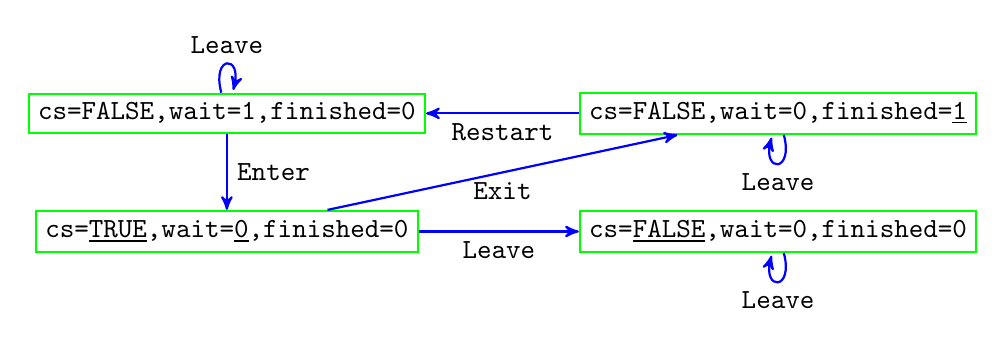
\begin{tikzpicture}[->,>=stealth',bend angle=45,auto,thick]

    \node[draw=green, node distance=7cm] (1) {\tt cs=FALSE,wait=1,finished=0};
    \node[draw=green, below of=1, node distance=1.5cm] (2) {\tt cs=\underline{TRUE},wait=\underline{0},finished=0};
    \node[draw=green, right of=2, node distance=7cm] (3) {\tt cs=\underline{FALSE},wait=0,finished=0};
    \node[draw=green, right of=1, node distance=7cm] (4) {\tt cs=FALSE,wait=0,finished=\underline{1}};

    %\node[above of=4, node distance=1cm] (ph) {};

    \path
    (1) edge[draw=blue] node{{\tt Enter}} (2)
    (2) edge[draw=blue,below] node{{\tt Leave}} (3)
    (2) edge[draw=blue,below] node{{\tt Exit}} (4)
    (4) edge[draw=blue] node{{\tt Restart}} (1)
    (1) edge[loop above,draw=blue] node{{\tt Leave}} (1)
    (3) edge[loop below,draw=blue] node{{\tt Leave}} (3)
    (4) edge[loop below,draw=blue] node{{\tt Leave}} (4);
\end{tikzpicture}
\caption{Mutex statespace for {\tt MAXINT=1}}
\label{fig:mutex}
\end{figure}

\end{document}
